% !TEX root = thesis.tex
\graphicspath{{./figures/}}

%%%%%%%%%%%%%%%%%%%%%%%%
\chapter{Implementation}
%%%%%%%%%%%%%%%%%%%%%%%%

The design above allows for multiple implementations, which will be introduced in this section. This section will also discuss briefly the robustness of the implementations, meaning how they respond to invalid input graphs. They will be explored and evaluated in section XX. Specifically, this paper will cover three implementations, which were chosen as they promise efficiency and scalability.

The implementations were coded in Python. Python is versatile, simple, and offers a large collection of helpful libraries like NetworkX, a library for working with graphs \cite{hagbergExploringNetworkStructure2008}. 

The algorithms take as input python dictionaries ("dicts"), as inputs, which map a key to a value \cite{pythonsoftwarefoundationPythonTutorialSection}. The delegation graph is represented in a "dict of dicts" format, where every key in the outer dict is a node, and the value is another dict, which has the node's neighbors as keys, and a weight as value. The algorithm's use as input "inverse" delegation graphs, where the inner dictionaries represent a node's incoming delegations rather than its outgoing edges. \Cref{fig:inverse_dict_example} shows an example of this. Considering that the standing power equations used in the system of linear equations list contain the incoming delegations for each node, this design choice improves efficiency as an algorithm can look up a node in the dictionary and learn about all its incoming delegations.

\begin{figure}[t]
    \centering
    \begin{subfigure}[t]{0.45\textwidth}
        \centering
        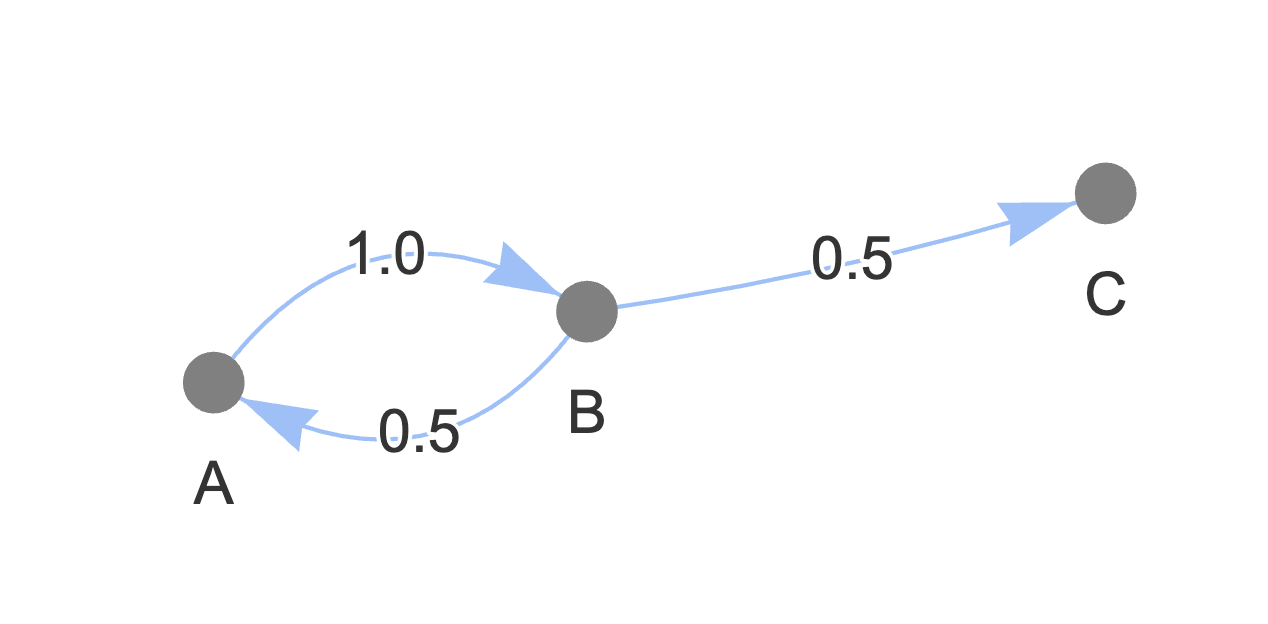
\includegraphics[width=\textwidth]{small_cycle_graph}
        \caption{Delegation graph}
    \end{subfigure}
    \hfill
    \begin{subfigure}[t]{0.45\textwidth}
        \centering
        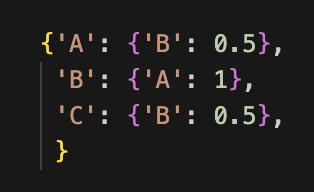
\includegraphics[width=\textwidth]{small_cycle_graph_inverse_dict}
        \caption{Inverse dict representation}
    \end{subfigure}
    \caption{Delegation graph and its inverse dict representation}
    \label{fig:inverse_dict_example}
\end{figure}

\section{Linear System Solver (LS)}

The first approach uses a dedicated linear system solver. We use SciPy's \texttt{scipy.sparse.linalg.spsolve} solver, which is optimized for sparse matrices \cite{virtanenSciPy10Fundamental2020}. A sparse solver is better equipped to resolve delegations if we assume that realistically each delegator only delegates to a few delegates. Since each $wp_v$ term in the system of linear equations can be mapped to one unique edge $(u, v, p) \in E$, the matrix corresponding to the system of linear equations likely has relatively few non zero entries compared to its size. In other words:

\[
\text{For a small } n \in \mathbb{N} \text{, and a large |V|}, D \subset V: n \cdot |D| < |V| \cdot |V|
\]

 \TODO{This explanation is ugly, but idk if its worth spending a lot more time on...} 
 
 The implementation makes use of SciPy's Compressed Sparse Column (CSC) arrays, which builds matrixes using $(x,y)$ coordinates and their corresponding data, which unless specified otherwise is 0 \cite{virtanenSciPy10Fundamental2020}. 

\TODO{This sentence below abt the perfect accuracy makes no sense atm, change it to fit into this section}
The solver solves the system of linear equations directly, using the SuperLU solver, so it is not possible to trade off runtime for accuracy, as done in the previous methods \cite{liSuperLUUsersGuide1999}. 

\section{Linear Programing Solver (LP)}

Secondly, we use the Python library PuLP, which provides an interface to Linear Programming (LP) solvers \cite{osullivanPuLPLinearProgramming2011}. To resolve the delegation graphs, we use the "Coin-or branch and cut" (CBC) solver, since it is free and open-source \cite{johnforrestCoinorCbcRelease2024}. Given the academic context and the moderate size of our delegation graphs, CBC provides a practical balance between performance and accessibility. Moreover, since our model essentially solves a system of linear equations with a unique correct solution, the choice of solver has little influence on the outcome itself — even if CBC is not the most optimized solver for this class of problems. While commercial solvers may offer faster runtimes, CBC is sufficient for our use case and ensures reproducibility without licensing constraints.

\TODO{The mention below abt the perfect accuracy makes no sense atm, since we have not introduced the iterative solver yet, change it to fit into this section}
The algorithm first sets up the linear program, setting up an equation $p'_v = \sum_{(u, v, w) \in E} 1 + wp'_u$ for each node $v \in V$. This is then solved by the CBC solver, with the primal tolerance set to $5*10^{-3}$ to level the playing field compared to the iterative algorithm, which does not have perfect accuracy either. A tolerance of $5 * 10^{-3}$ assures that $\lvert p'_v -\sum_{(u, v, w) \in E} 1 + wp'_u \rvert \le 5*10^{-3}$, so the solutions will be correct when rounded to the second decimal place \cite{forrestCBCUserGuide2005}. Finally, the algorithm cleans the $p_v'$ values, setting any delegators power to 0. 


\TODO{Add links to the implementations on GitHub}

\section{Iterative Solver (Iterative)}

The iterative solver aims to leverage the format of the input, and eliminate any necessary overhead. It is based on the Jacobi method of solving systems of linear equations, which solves the system by iteratively refining the solution \TODO{cite}, however we will prioritize an intuitive explanation of the procedure.

\subsection{Approach}

A delegation can be thought about as liquid throwing through a graph. Each delegator is a "source", and power flows from its source between nodes until it eventually ends in a sink. If a delegator A delegates half their vote to B and the other half to other nodes, half of A's power should flow to B. An algorithm should thus add 0.5 to Bs power, and remove it from A. If B is a sink, the algorithm is done resolving this delegation. However,  B may not be a sink, in which case, the power continues to flow further, to B's delegates. An algorithm would need to iterate over the graph multiple times, until an equilibrium has been reached, where all power in the graph has flown into a sink. \Cref{alg:iterative_simple} shows such an algorithm drafted in pseudocode. Each iteration, a snapshot of the power's of each node is taken, and the reassignments of power are based on this snapshot\footnotemark.  

\footnotetext{If the algorithm forwent the use of such a snapshot, it would lead to inconsistencies in the edge case of a self-delegation of weight less than 1, since the self-delegator's power would change in the middle of reassigning the power. This is also how the Jacobi method approaches this challenge. Each iteration, a solution vector containing intermediate results is created, and passed as input into the next iteration.}

Another valid approach would be a queue-approach, where the algorithm pops node off a queue and delegates their power, and each delegate of this node gets re-added to the queue. A sweeping method treating the entire graph at once was chosen due to its increased simplicity and runtime analysis.

\begin{algorithm} [H]
 \caption{Iterative Algorithm}\label{alg:iterative_simple}
\begin{algorithmic}[1]
\State // Initialize each node’s power to 1.0  
\ForAll{\(v \in \texttt{nodes}\)}
    \State \(\texttt{powers}[v] \gets 1.0\)
\EndFor
\Repeat
    \State \(\texttt{prev\_powers} \gets \texttt{powers}.\texttt{copy}()\)  \Comment{snapshot of previous iteration}
    \ForAll{\(v \in \texttt{nodes}\)}
        \State // For each incoming delegation \((u \to v)\), move \(w_{uv}\times\) previous power of u
        \ForAll{\((u, w) \in \texttt{delegations}[v]\)}
            \State \(\delta \gets w \times \texttt{prev\_powers}[u]\) \label{alg:iterative_simple_delta_assignment}
            \State \(\texttt{powers}[u] \;-\!=\; \delta\) \label{alg:iterative_simple_remove_delta}
            \State \(\texttt{powers}[v] \;+\!=\; \delta\) \label{alg:iterative_simple_add_delta}
        \EndFor
    \EndFor
\Until{\(\texttt{prev\_powers} = \texttt{powers}\)} \label{alg:iterative_simple_termination_cond}\Comment{a steady state has been reached}
\end{algorithmic}
\end{algorithm}

The following notation will be used throughout the next sections.

$G = (V, E)$ is a well-formed delegation graph, with $V = D \dot\bigcup S$, where D is the set of delegators and S is the set of sinks.

Let $p_v^{(i)}, i \in \mathbb{N}_0$ be \texttt{powers}[v] after the $i$-th iteration of the repeat-until loop, with $p_v^{(0)}$ being the initial power of a node before the first iteration has started. Using this notation, our termination condition for the repeat-until loop at \cref{alg:iterative_simple_termination_cond} of \cref{alg:iterative_simple} is: $\forall v \in V: p_v^{(i-1)} = p_v^{(i)}$

Let $P_D^{(i)} = \sum_{d \in D} p_d^{(i)}$ and $P_S^{(i)} = \sum_{s \in S} p_s^{(i)}$ be the sums of all delegators and all sinks after each iteration.

Let $\delta_{(u, v, w)}^{(i)} = w * p_v^{(i)}$ be the delta assigned in \cref{alg:iterative_simple} at \cref{alg:iterative_simple_delta_assignment} during the $i$th iteration.


\subsection{Conservation of Power}

We show, that this algorithm conserves power throughout iterations. This insight .... XXX \TODO{here}

\begin{theorem}
\label{theo:iterative_cons_of_power}
Given a well-formed delegation graph, in \cref{alg:iterative_simple}, $P_t^{(i)} = P_D^{(i)} + P_S^{(i)}$ is equal to $|V|$ for any $i \in \mathbb{N}_0$.
\end{theorem}
\begin{proof}

We prove the theorem inductively. When $i = 0$ (before the first iteration), each node is assigned a power of 1. So 

\[
\forall v \in V: p_v^{(i)} = 1 \implies P_t^{(0)} = |V|
\]

Assume that for a $k \in \mathbb{N}_0: P_t^{(k)} = |V|$. During iteration $k+1$, the algorithm will iterate over all delegations, and for each $(u, v, w) \in E$, it will remove some $\delta_{(u, v, w)}^{(k+1)}$ from node \texttt{u} in \cref{alg:iterative_simple_remove_delta}, but add this same amount to node \texttt{v} in \cref{alg:iterative_simple_add_delta}. Since the delegation graph is well formed, the outgoing weights of any delegator add up to 1, so for all delegators $u \in D$, the total amount of power they delegate away during iteration $k+1$ adds up to the power they held in iteration $k$.

\begin{align*}
\sum_{(u, v, w) \in E} \delta_{(u, v, w)}^{(k+1)} &=  \sum_{(u, v, w) \in E} wp_u^{(k)} \\
&= p_u^{(k)}  \sum_{(u, v, w) \in E} w \\
&= p_u^{(k)} \cdot 1 \\
&= p_u^{(k)}
\end{align*}

Thus, throughout the iteration of the outer loop, any delegator $u$ only ever moves power it already has, and for each "moving around" of power, conservation is guaranteed since any power subtracted from a delegator is re-added to the delegate. This means that power is only ever moved around, but not lost, and $P_t^{(k+1)} = |V|$. 

By the principles of induction, the assumption holds for any $i \in \mathbb{N}_0$
\end{proof}

\subsubsection{Similarity to the Previous Approach}

Observing the algorithm reveals that the same equations used in the previous approach to resolve delegations can be re-found here. Algorithm starts with a vector of ones, indicating an initial power of each node of one. Furthermore, each iteration, each node $u \in V$ gains power amounting to $\sum_{(u, v, w) \in E} \delta^{(i)}_{(u, v, w)}$. This term can be rearranged as follows:

\begin{align*}
p_v^{(i)} &+= \sum_{(u, v, w) \in E} \delta^{(i)}_{(u, v, w)} \\
&+= \sum_{(u, v, w) \in E} wp_v^{(i-1)}
\end{align*}

Since power is conserved, the same amount is also removed from the node, thus we can say, that

\[
p_v^{(i)} = \sum_{(u, v, w) \in E} wp_v^{(i-1)} \forall v \in V
\]


This is the same al the standing power assigned to all nodes in the previous approach. ($p'_v = 1 + \sum_{(u, v, w) \in E} wp'_u$). Thus, this algorithm solves the same problem as the system of linear equations introduced in the previous section. 

\TODO{This section may still be missing an explanation of the jacobi method. I proved that each iteration I resolve something resembling the initial system of linear equations method, but since the reader does not know the jacobi method, they might not be able to notice the similarity.}

\subsubsection{Implementation}

This section will show, that the algorithm does not necessarily terminate despite input with a well formed delegation graph, after which we propose an amended algorithm.

First, we prove that a sink's power can't shrink, since there is no outgoing edge going out of a sink.

\begin{lemma}\label{lem:sink_non_shrink}
$\forall s \in S: p_s^{(i)} \ge p_s^{(i-1)}$ 
\end{lemma}
\begin{proof}
Assume $p_s^{(i)} < p_s^{(i-1)}$. The power that left $s$ needs to have gone somewhere, since the algorithm conserves power. This implies, that there is a delegation $(s, v, w) \in E$ such that $\exists \delta > 0: \delta \gets w * p_s^{(i-1)}$. This contradicts our definition of a well-formed liquid delegation graph, since any sink can not have any outgoing edges.
\end{proof}

Next, we prove that if a node's power is 0, all its delegator's powers must have been 0 after the previous iteration
\begin{lemma}\label{lem:simple_iterative_empty_node}
$p_v^{(i)} = 0 \implies \forall (u, v, w) \in E: p_u^{(i - 1)} = 0$. 
\end{lemma}
\begin{proof} Assume $p_v^{(i)} = 0$, but $\exists (u, v, w) \in E: p_u^{(i-1)} > 0$

Let $d \in \mathbb{R}_{0}$ be any additional power a node receives, that is not explicitly mentioned.

\[
p_u^{(i-1)} > 0 \implies \delta_{(u, v, w)}^{(i)} > 0 \implies p_v^{(i)} = \delta_{(u, v, w)}^{(i)} + d \implies p_v^{(i)} > 0 \lightning
\]

\end{proof}

Next, we prove that the algorithm terminates at iteration $i+1$ exactly when $P_D^{(i)} = 0$.

\begin{lemma}\label{lem:simple_alg_terminates}
 $p_v^{(i)} = p_v^{(i+1)} \forall v \in V \Leftrightarrow$ $P_D^{(i)} = 0$.
\end{lemma}
\begin{proof}

\begin{align*}
	P_D^{(i)} = 0 
	&\Leftrightarrow p_d^{(i)} = 0, \forall d \in D \\
	&\Leftrightarrow \not\exists (d, v, w) \in E: \delta_{(d, v, w)}^{(i+1)} > 0  &&\text{($\delta$ of a node with power 0 is 0)}\\
	&\Leftrightarrow p_v^{(i)} = p_v^{(i+1)} \forall v \in V \qed  &&\text{($p_v$ doesn't change if zero is added to it)}
\end{align*}
\end{proof}

\begin{theorem}\label{alg:iterative_alg_doesnt_terminate}
Given a well-formed delegation graph, \cref{alg:iterative_simple} may not terminate.
\end{theorem}
\begin{proof} Assume the algorithm terminates on a well-formed delegation graph..

Take the following well formed delegation graph $G = (S \dot\bigcup D, E)$with $S =\{C\}$ and $D = \{A, B\}$. B delegates half their vote to A, and half their vote to C, while A delegates its entire vote back to B. Since the algorithm terminates, there must be an $i \in \mathbb{N}$ such that $P_D^{(i)} = 0$. 

\begin{figure}[h]
    \centering
    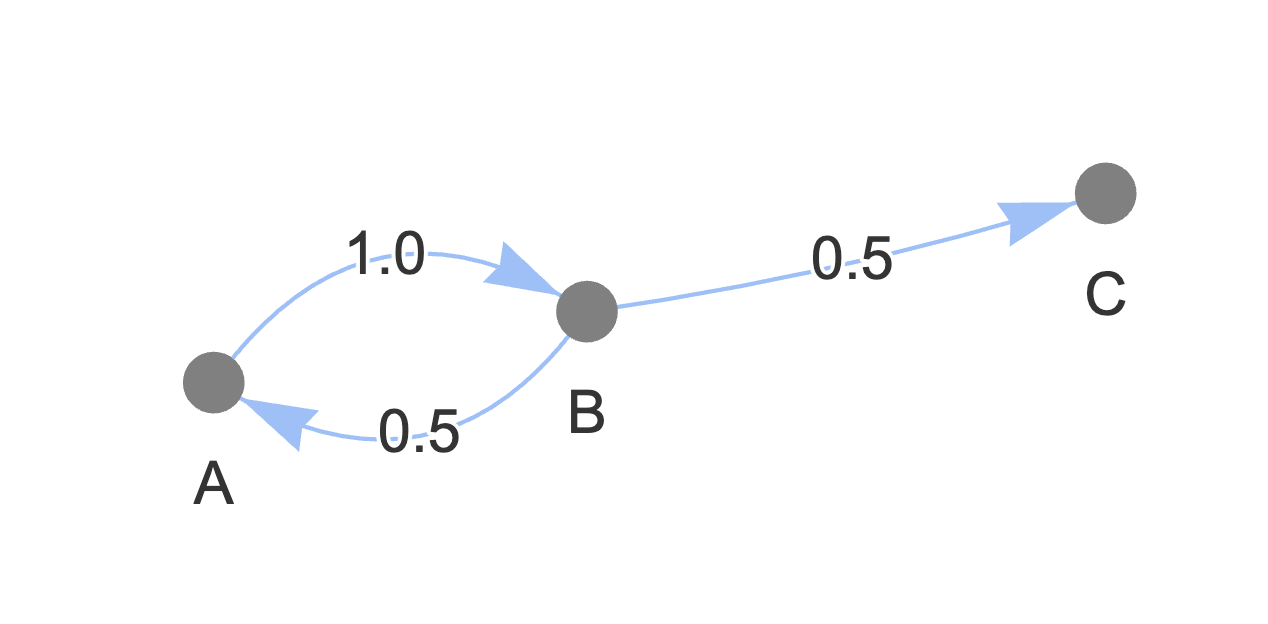
\includegraphics[width=0.4\textwidth]{small_cycle_graph}
    \caption{Delegation graph with a cycle.}
    \label{fig:small_cycle_graph}
\end{figure}


Both (B, A, 0.5) and (A, B, 1) $\in E$, so A is a predecessor of B, and B is a predecessor of A, thus B is its own predecessor.

\begin{align*}
	P_D^{(i)} = 0 
	&\implies p_B^{(i)} = 0 \\
	&\implies p_A^{(i-1)} = 0 &&\text{(Lemma \cref{lem:simple_iterative_empty_node})} \\
	&\implies p_B^{(i-2)} = 0 &&\text{(Lemma \cref{lem:simple_iterative_empty_node})}
\end{align*}

This implication chain can be drawn arbitrarily long. In order for B to have a power of 0, it can never have held any power in the first place, contradicting our well-formed delegation graph, which dictates that all nodes start with a power of 1.
\end{proof}

If the graph is acyclic, this algorithm would need at most $|V|$ iterations, such as in a directed path, where each node gives their entire vote to the next node except for the final sink. However, as soon as cycles are introduced into the graph, the spreading of power only terminates after an infinite amount of steps. Looking further into the graph in \cref{fig:small_cycle_graph}, the expected resolution of these delegations would be that C holds node A and B's powers, as well as its own initial vote, so a power of three. However, looking at the powers as the algorithm iterates over this graph reveals that after the first iteration, C will have 1.5 votes, then 2, then 2.25, 2,50, 2.75, ..., however only after infinitely many steps it will have three. 

\begin{table}[h]
  \centering
  \caption{$p_v{(i)}$ values of nodes in the graph in \cref{fig:small_cycle_graph}}
  \label{tab:simple_iterative_example}
  \begin{tabular}{| l | l | l | l |}
    \hline
    i & $p_A$ & $p_B$ & $p_C $ \\ \hline
    0 & 1 & 1 &	1 \\ \hline
    1 & 0.5 & 1 & 1.5 \\ \hline
    2 & 0.5 & 0.5 & 2 \\ \hline
    3 & 0.25 & 0.5 & 2.25 \\ \hline
    4 & 0.25 & 0.25 & 2.50 \\ \hline
    5 & 0.125 & 0.25 & 2.625 \\ \hline
    \multicolumn{4}{| l |}{...} \\ \hline
  \end{tabular}
\end{table}

Practically, the algorithm needs a cutoff condition, which terminates the while loop once the power values calculated are close enough to the real, final values. Since these are unknown before the algorithm terminates, we can count how much power is being shifted throughout the graph each iteration, and terminate once this value is sufficiently small. An extension to \cref{alg:iterative_simple} could look like \cref{alg:iterative_with_cutoff}. 

\begin{algorithm} [H]
 \caption{Iterative Algorithm with a cuttoff value. Changes from \cref{alg:iterative_simple} are highlighted. }\label{alg:iterative_with_cutoff}
\begin{algorithmic}
\State // Initialize each node’s power to 1.0  
\ForAll{\(v \in \texttt{nodes}\)}
    \State \(\texttt{powers}[v] \gets 1.0\)
\EndFor
\Repeat
    \State \(\texttt{prev\_powers} \gets \texttt{powers}.\texttt{copy}()\) 
    \State \colorbox{yellow}{\(\texttt{total\_change} \gets \texttt{0}\)} 
    \ForAll{\(v \in \texttt{nodes}\)}
        \State // For each incoming delegation \((u \to v)\), move \(w_{uv}\times\) previous power of u
        \ForAll{\((u, w) \in \texttt{delegations}[v]\)}
            \State \(\delta \gets w \times \texttt{prev\_powers}[u]\)
            \State \(\texttt{powers}[v] \;+\!=\; \delta\)
            \State \(\texttt{powers}[u] \;-\!=\; \delta\)
            \State \colorbox{yellow}{\(\texttt{total\_change} \;+\!=\; \delta \)}
        \EndFor
    \EndFor
\Until{\colorbox{yellow}{\(\texttt{total\_change} < \texttt{cutoff}\)}}
\end{algorithmic}
\end{algorithm}

\subsubsection{Conservation of Power}

\Cref{theo:iterative_cons_of_power} states that \cref{alg:iterative_simple} conserves power across iterations. The same proof applies to \cref{alg:iterative_with_cutoff}, since only the if-condition of the outer loop has changed, but the algorithm works the same way. So while the algorithm will iterate less, power remains conserved across iterations.

\subsubsection{Termination}

\begin{lemma}\label{lem:iterative_alg_power_concentrates}
Given a well-formed delegation graph, \cref{alg:iterative_with_cutoff} terminates if \texttt{cutoff} > 0.
\end{lemma}

\TODO{The proof is incomplete, I'll work over it later...}

\begin{proof} We differentiate two cases. Fix an $i \in \mathbb{N}_0$.

Case 1: $P_D^{(i)} = 0$

In this case, no delegator has any power, so the \texttt{total\_change} can be at most 0, which is always smaller than \texttt{cutoff}. So the algorithm terminates.

Case 2: $P_D^{(i)} > 0$

\begin{align*}
P_D^{(i)} > 0 
& \implies \exists d_0 \in D: p_{d_0}^{(i)} > 0 \\ 
& \implies \exists s \in S, \exists k \ge 1, \exists (v_0, ..., v_k): v_0 = d_0, v_k= s, (v_j, v_{(j+1)}, w) \in E \forall 0 \le j \le k \\
&\text{(There is a path between $d_0$ and a sink)} \\
& \implies \exists d_{k-1} \in D: (d_{k-1}, s, w) \in E \\
& \text{($d_{k-1}$ is the node on the path from $d_0$ to $s$ that has an edge to $s$)}
\end{align*}

Assume ${p_{d_{k-1}}}^{(i)} = 0$.

Left $\mathrm{Pred}^*(d_0)$ be defined as follows:

\[
\mathrm{Pred}^*(d_{0})=\bigl\{u \in V \bigm| \exists\text{ a path }u \rightsquigarrow d_{0} \bigr\}
\]

Also, let $\mathrm{dist}(d_{0}, p), p \in V$  be defined as follows :

\[
\mathrm{dist}(d_{0},p) =\min\bigl\{|P| : P\text{ is a path }d_{0}\rightsquigarrow p\bigr\}.
\]

\begin{align*}
{p_{d_{k-1}}}^{(i)} = 0 &\implies 
\end{align*}

$\max\bigl\{\mathrm{dist}(d_0,p)\bigm|p\in \mathrm{Pred}^*(d_0)\bigr\} $

...

%{p_{d_{(k-1)}}}^{(i)} = 0

%The algorithm assumes, that the \texttt{total\_change} eventually shrinks below the cutoff value. 

\TODO{todo continue here, I am too lazy atm to try and figure out how to prove that P\_D shrinks properly}

\end{proof}


\section{Robustness}

This section describes the different implementations behavior when a delegation graph is not well formed. Specifically, their behaviors when outgoing delegation weights are invalid, so not adding up to 1, and if the delegation graph contains a closed delegation cycle. 

\subsection{Invalid delegations}

On their own, neither of the three implementations will definitively cause an error when delegations are invalid. The iterative implementation is "dumb", in the sense that it moves around power as it finds them in the delegations. If a delegator delegates more than they are meant to, the algorithm behavior becomes undefined, since the delegators power may become negative, at which point the delta in power calculated from its power also becomes negative, which messes with the \texttt{total\_change} value in unpredictable ways. 

If a delegate delegates less than their vote, this causes less of an issue. As long as the delta calculated at $\delta \gets w \times \texttt{prev\_powers}[u]$ does not become negative, the algorithm's behavior becomes quite predictable. A well-formed delegation graph is allowed to contain self-delegations as long as their weight is lower than 1, such as the delegation in \cref{subfig:permissible-self-delegation}. In this situation, power still leaves the node, but less slowly. When the iterative algorithm goes over the graph, not delegating enough weight has the same effect as such a self-delegation, since in the former situation  power gets subtracted and then re-added to the node, while in the latter it just remains untouched.

\begin{figure}[h]
    \centering
    \begin{subfigure}[t]{0.45\textwidth}
	\centering
	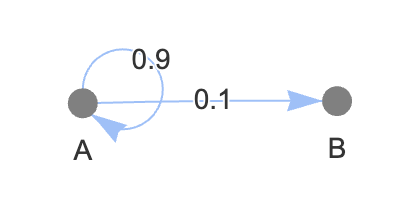
\includegraphics[width=0.9\textwidth]{allowed_self_loop}
	\caption{Permissible delegation graph}
	\label{subfig:permissible-self-delegation}
    \end{subfigure}
    \hfill
    \begin{subfigure}[t]{0.45\textwidth}
        \centering
        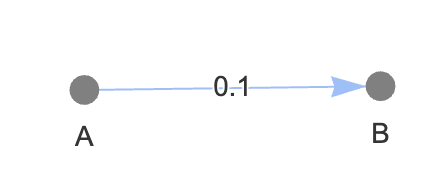
\includegraphics[width=\textwidth]{invalid_delegation_graph}
        \caption{Invalid delegation graph}
         \label{subfig:invalid-delegation-graph} 
    \end{subfigure}
    \caption{Two similar delegation graphs}
    \label{fig:small-delegation-graphs}
\end{figure}

For the two implementations directly based on solving systems of linear equations, this is a little different. Node \texttt{B}'s power would end up as 1.1, since the system of linear equations looks as follows:

\begin{align*}
& p_A = 1 \\
& p_B = 1 + 0.1p_A
\end{align*}

As long as the delegations form a matrix that is singular, there will be a unique solution, so even with invalid delegations, the algorithm will find power values, however they most likely differ whom the power values that would be expected, and probably not conserve total power properly. 

\subsection{Closed Delegation Cycles}

If the delegations form a closed delegation cycle, the iterative algorithm will not terminate, since the algorithm will iterate any power that is in or enters the cycle around the cycle indefinitely. 

For the other two algorithms however, such a cycle can be caught. The equations for the standing power of the nodes within the cycle are linearly dependent on each other, thus the matrix resulting from them is not singular, and hence don't have a single solution. Solvers of systems of linear equations catch and throw an error. Similarly, the LP solver will find that the linear program is infeasible.

What is worth mentioning however, is that since we allow fractional delegation, it suffices if just one node is a closed delegation cycle does also delegates to a node outside of a delegation cycle (or turns into a sink), for the delegations to become resolvable again. The cycles that were explored in \cref{subsec:cycles_draining} are example of such a situation. 


